Dette kapitel evaluerer de to valgte sensormodeller (\cref{mapping:sensormodel}).
\thilemann{lidt fesen intro, men måske svær at gøre mere interessant...}

\section{Formål}
Formålet med denne test er at se hvilken sensormodel, der kommer frem til det mest præcise kort.
Dette er for at se om målsætningen beskrevet i \cref{problem:maalsaetning} er opfyldt.\thilemann{Er det kun mig som har problemer med denne henvisning?}

\section{Vurderingsmål}
Da alle tests vil returnere et helt eller delvist udfyldt occupancy grid, vil sammenligningen gå ud fra dette.
Alle grids, som er resultat af en test, vil blive sammenlignet med et optimalt occupancy grid (lavet ud fra fysisk observation).
Ethvert grid (både test og optimalt) vil bestå af tre typer celler:
\thilemann{Vi skriver tidligere i rapporten om at celler kan vær \textit{occupied} og \textit{free} - vi bør være konsekvente og kun benytte danske termer}
\begin{description}
\item[Optaget]{ er en celle, hvor der er en forhindring.}
\item[Fri]{ er en celle, der er vurderet som fri, enten gennem måling eller ved at robotten er kørt hen over den.}
\item[Ukendt]{ er en celle, hvor om der ikke er opnået viden.
For det optimale grid, vil det være celler inde i en større forhindring.
For et test grid, kan det være det samme som for det optimale, dog kan der også forekomme ukendte celler, som skulle have været enten frie eller optagede.}
\end{description}

\subsection{Sammenligning}
For enhver celle i et test grid, vil denne blive sammenlignet med den tilsvarende celle i det optimale grid.
Der vil være i alt 9 scenarier, da enhver celle har 3 tilstande.
I \cref{evaluering:sammenligning} kan resultatet af denne sammenligning ses.

\begin{table}[h]
\centering
\begin{tabular}{|l|c|c|c|}
\hline
Test \textbackslash~Optimalt & Optaget & Fri & Ukendt \\ \hline
Optaget & $+1$ & $-1$ & $0$ \\ \hline
Fri & $-1$ & $+1$ & $0$ \\ \hline
Ukendt & $-1$ & $-1$ & $0$ \\ \hline
\end{tabular}
\caption{Resultater for sammenligning af test grid celle og optimalt grid celle.}
\label{evaluering:sammenligning}
\end{table}

\subsection{Resultat}
Resultatet for et enkelt test grid vil være en akkumulering af sammenlignings-værdierne for cellerne.
Derved kommer der et enkelt tal for enhver test, hvorfor disse efterfølgende let kan sammenlignes.

\section{Test}\label{evaluering:test_beskrivelse}
Der bliver foretaget tre tests med hver sensormodel (\cref{mapping:sensormodel}).
I alle test benyttes ruteplanlægning beskrevet i \cref{ruteplanleagning}.
Robotten kører hen til et punkt og scanner to gange - dette foretages 75 gange.
Alle data bliver logget, så det er muligt at genskabe et kort udfra det.
Opstillingen af testen er beskrevet i \cref{evaluering:opstilling}

\subsection{Opstilling}\label{evaluering:opstilling}
Testmiljøet er beskrevet i \cref{testmiljo}.
Selve opstillingen til testen kan man se på \cref{evaluering:emptyGrid}, her kan man desuden se robottens startposition, som er den samme i alle tests.

\begin{figure}[h]
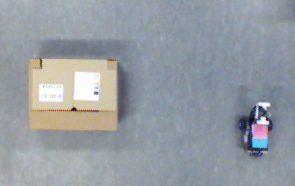
\includegraphics[width=\textwidth]{emptyGrid}
\caption{Forsøgsopstillingen inden hver test sættes i gang.}
\label{evaluering:emptyGrid}
\end{figure}
\subsection{Resultater}

\subsection{Opsummering}